\only<beamer>{\titleframe}

\author{SEA 2025 \hspace{1cm} Johanna Hofmann}
\section{Introduction}

% TODO: letzte Folie, full url
%  https://medium.com/@teamtechsis/introduction-to-sorting-algorithms-1623b9cdd4f1
% https://www.geeksforgeeks.org/dsa/quick-sort-algorithm/

\begin{frame}{The Selection Problem}
  \framesubtitle{Finding the $i$-th Smallest Element}
  \textbf{Selection($n,i$):} Find the $i$-th smallest element in a collection of $n$ distinct values.
  \vfill
  \centering
  Common approaches are based on sorting or partitioning:
  \begin{columns}[T]
    \begin{column}{0.45\textwidth}
      \centering
      \textbf{Sorting}\\
      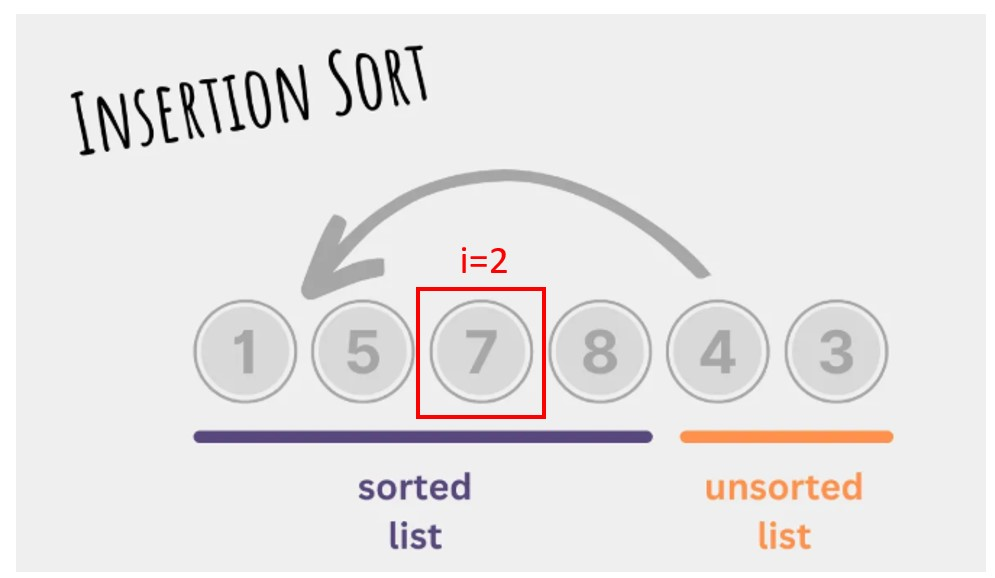
\includegraphics[width=0.8\textwidth, trim={0 0 0 3.5cm}, clip]{figures/Insertion_sort.jpg}\\
      \tiny{Source: medium.com/@teamtechsis}
    \end{column}
    \begin{column}{0.45\textwidth}
      \centering
      \textbf{Pivoting}\\
      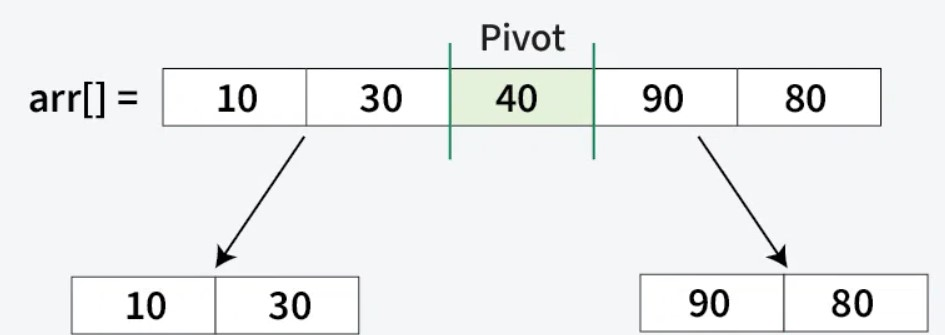
\includegraphics[width=0.8\textwidth]{figures/Pivot.jpg}\\
      \tiny{Source: geeksforgeeks.org}
    \end{column}
  \end{columns}

  \note{
    \begin{itemize}
      \item We concerned ourselves with finding exact lower bounds for the number of comparisons in the selection problem
      \item First of all, what is the Selection Problem?
      \item It can be defined by the task of finding the $i$-th smallest element in a collection of $n$ distinct values.
      \item All baseline algorithms are based on the principle of either sorting or pivoting. 
      \item I suppose you are familiar with the bubble sort algorithm or insertion sort. With sorting the list first and then just picking the selection problem can be solved in a trivial way.
      \item On the other hand, with pivoting one can leverage the advantages of divide-and-conquer and apply the well-known Quickselect algorithm or the median of medians appraoch.
    \end{itemize}
  }
\end{frame}

% TODO: diese Folie hat viel zu viel Text
\begin{frame}{Complexity of the Selection Problem}
  \framesubtitle{Known Asymptotic Bounds}
  \begin{itemize}
    \item<+-> Let $V_i^n$ be the worst-case number of comparisons for an optimal algorithm.
    \item<+-> Selecting the minimum is simple: $V_1(n) = n-1$.
    \item<+-> The best-known upper bound for selecting the median is $\approx 2.95n$ comparisons.
    \item<+-> The best-known lower bound for the median is $\approx 2.41n$ comparisons.
  \end{itemize}
  \note{
    \begin{itemize}
      \item By counting the comparisons during runtime one obtains the $i$-the smallest element end the number of comparisons at the same time.
      \item Let $V_i^n$ be the worst-case number of comparisons for an optimal algorithm.
      \item First, we accumulated known bounds.
      \item E.g. a lower bound for the general selection problem, is the number of comparisons needed for selecting the smallest element.
      \item That is just $n-1$
      \item The hardest element to determine is the median.
      \item The best-known lower bound for the median is $\approx 2.41n$ comparisons.
      \item The best-known upper bound for selecting the median is $\approx 2.95n$ comparisons.
      
    \end{itemize}
  }
\end{frame}

\begin{frame}{Complexity of the Selection Problem}
  \begin{figure}
    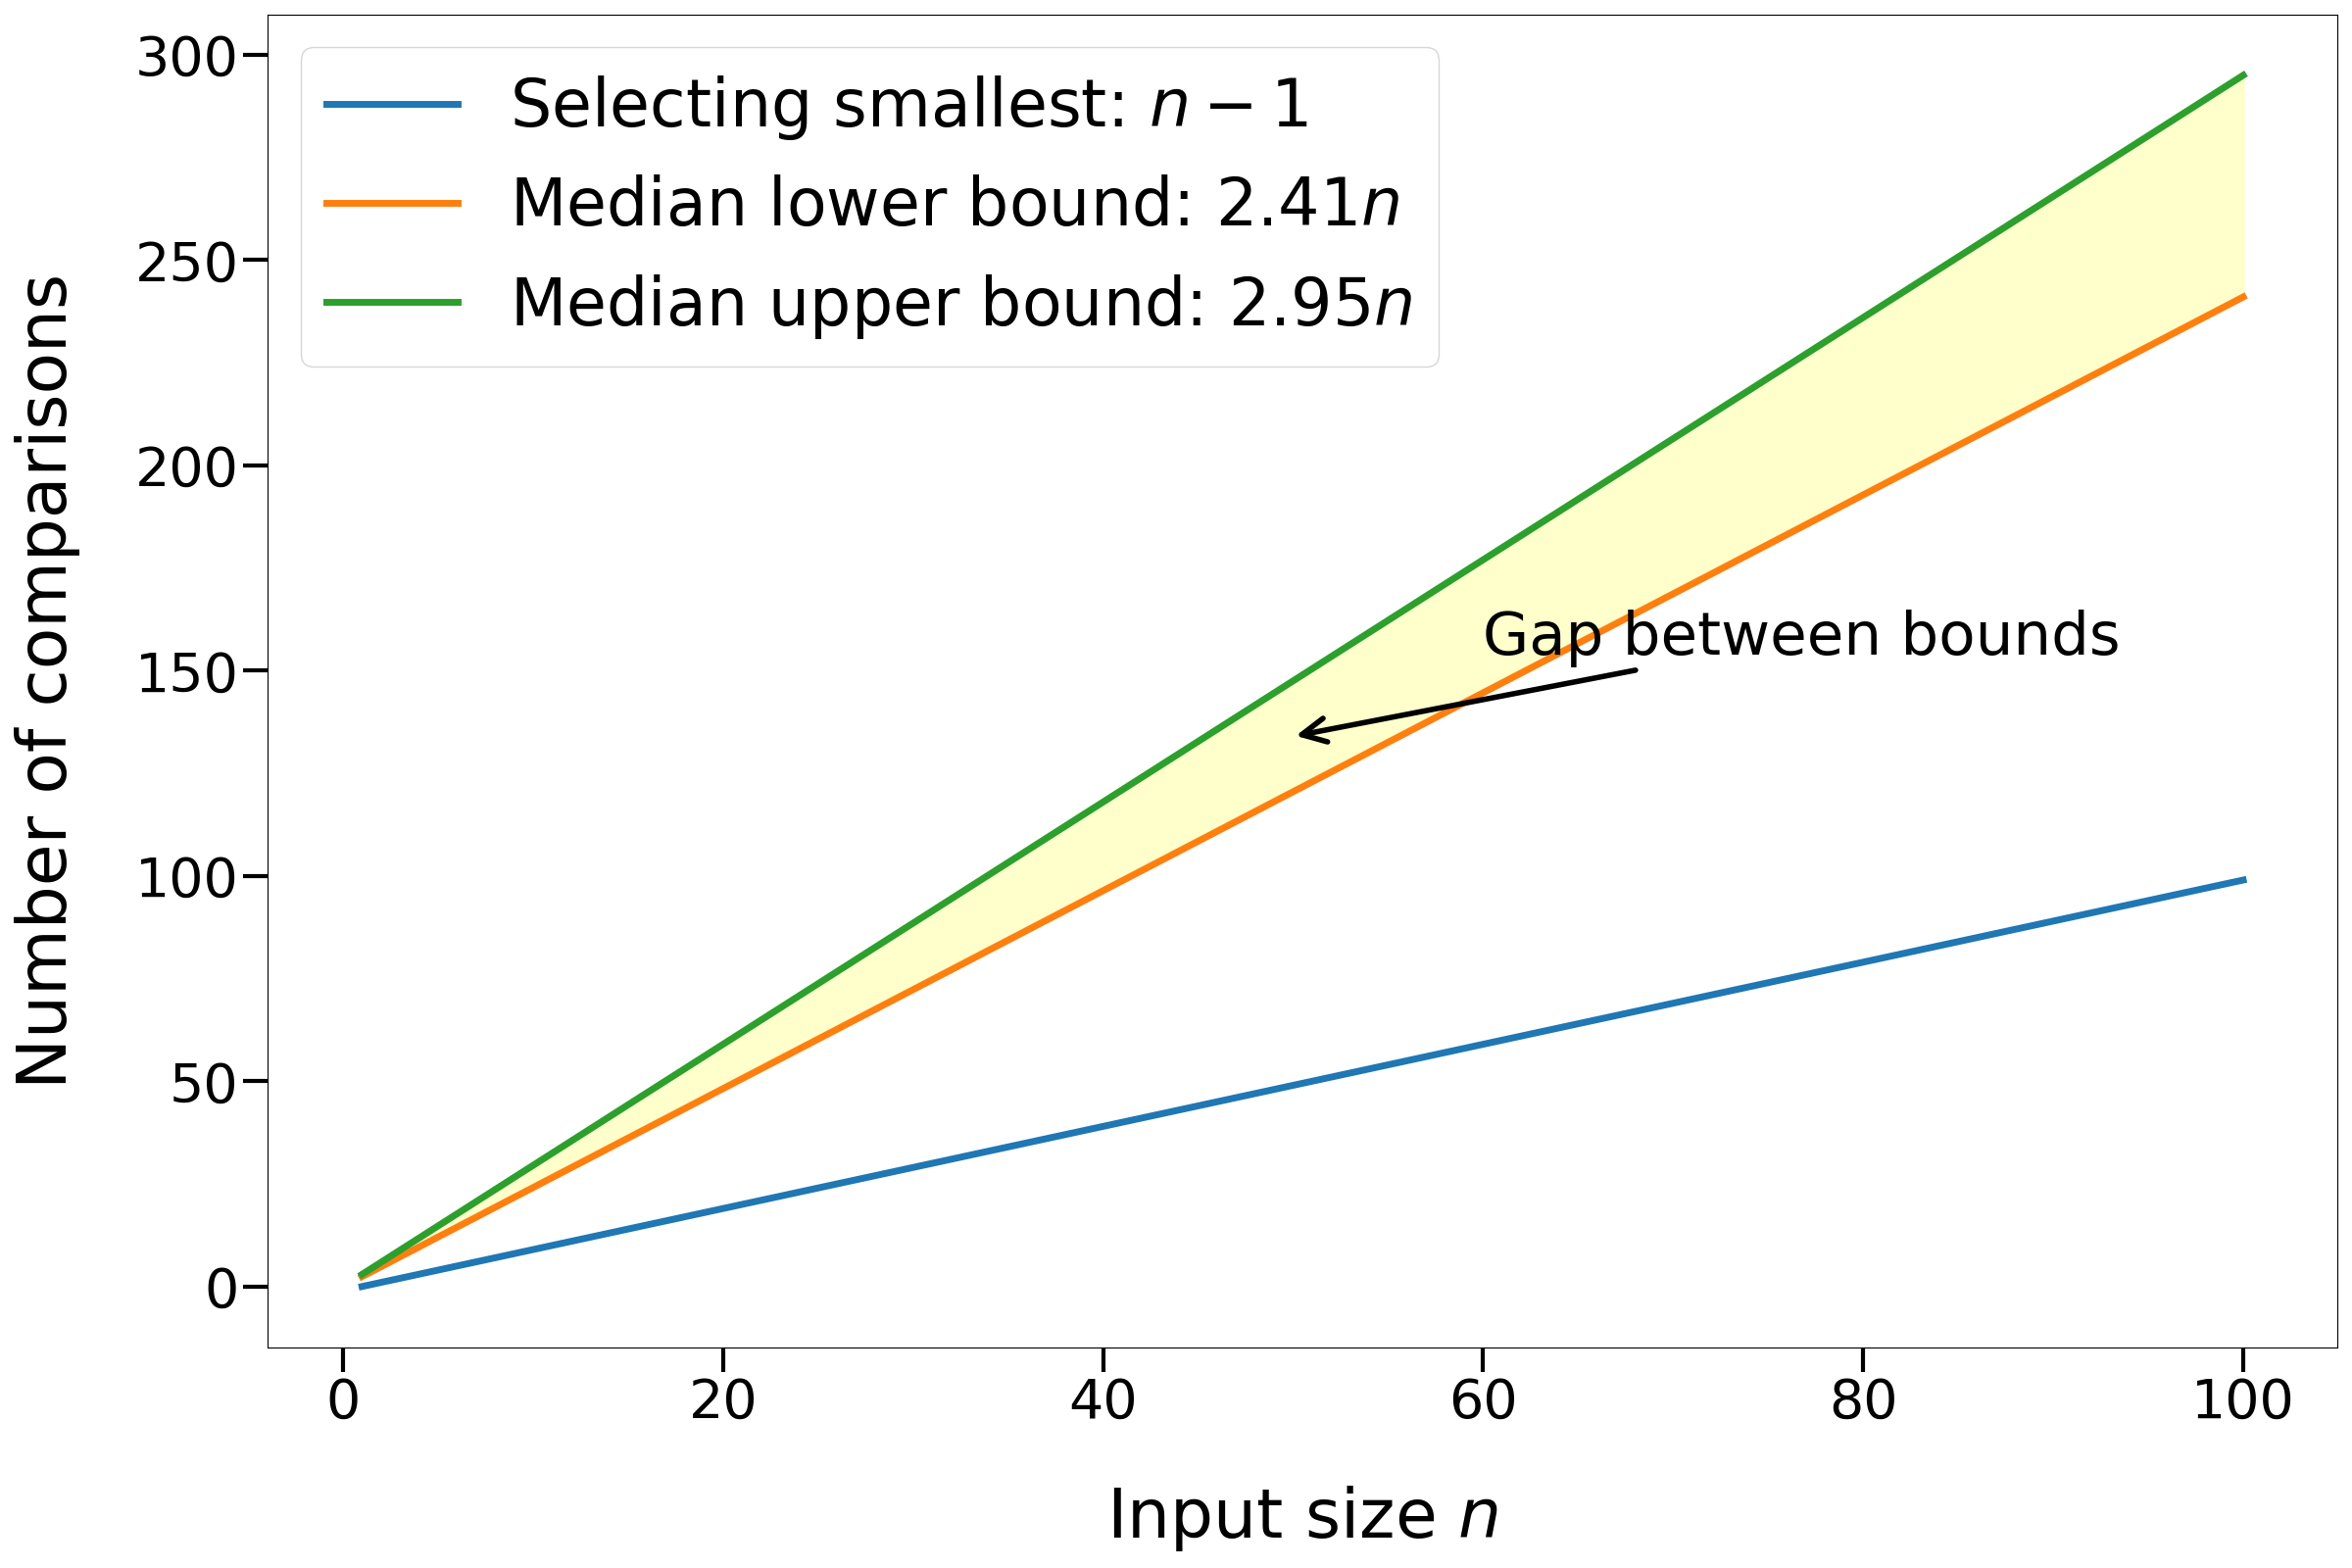
\includegraphics[height=0.75\textheight]{figures/bounds_diagram.png}
    \caption{\scriptsize Complexity Bounds for the Selection Problem}
  \end{figure}
  \note{
    \begin{itemize}
      \item Let's visualize that
      \item The green line represents for the numer of comaparions for selecting the smallest element
      \item The orange line represents the lower bound for the median
      \item The blue line represents the upper bound for the median
      \item We are intereseted in the gap between these existing bounds especially for small n's
      \item We explore, how many comparisons are needed for larger i's in contrast to $i=0$
      \item And also establish optimal algorithms for all $i$ and $n$ and therefore tighten the gap between upper and lower bounds.
    \end{itemize}
  }
\end{frame}

\begin{frame}{Complexity of the Selection Problem}
  \begin{figure}
    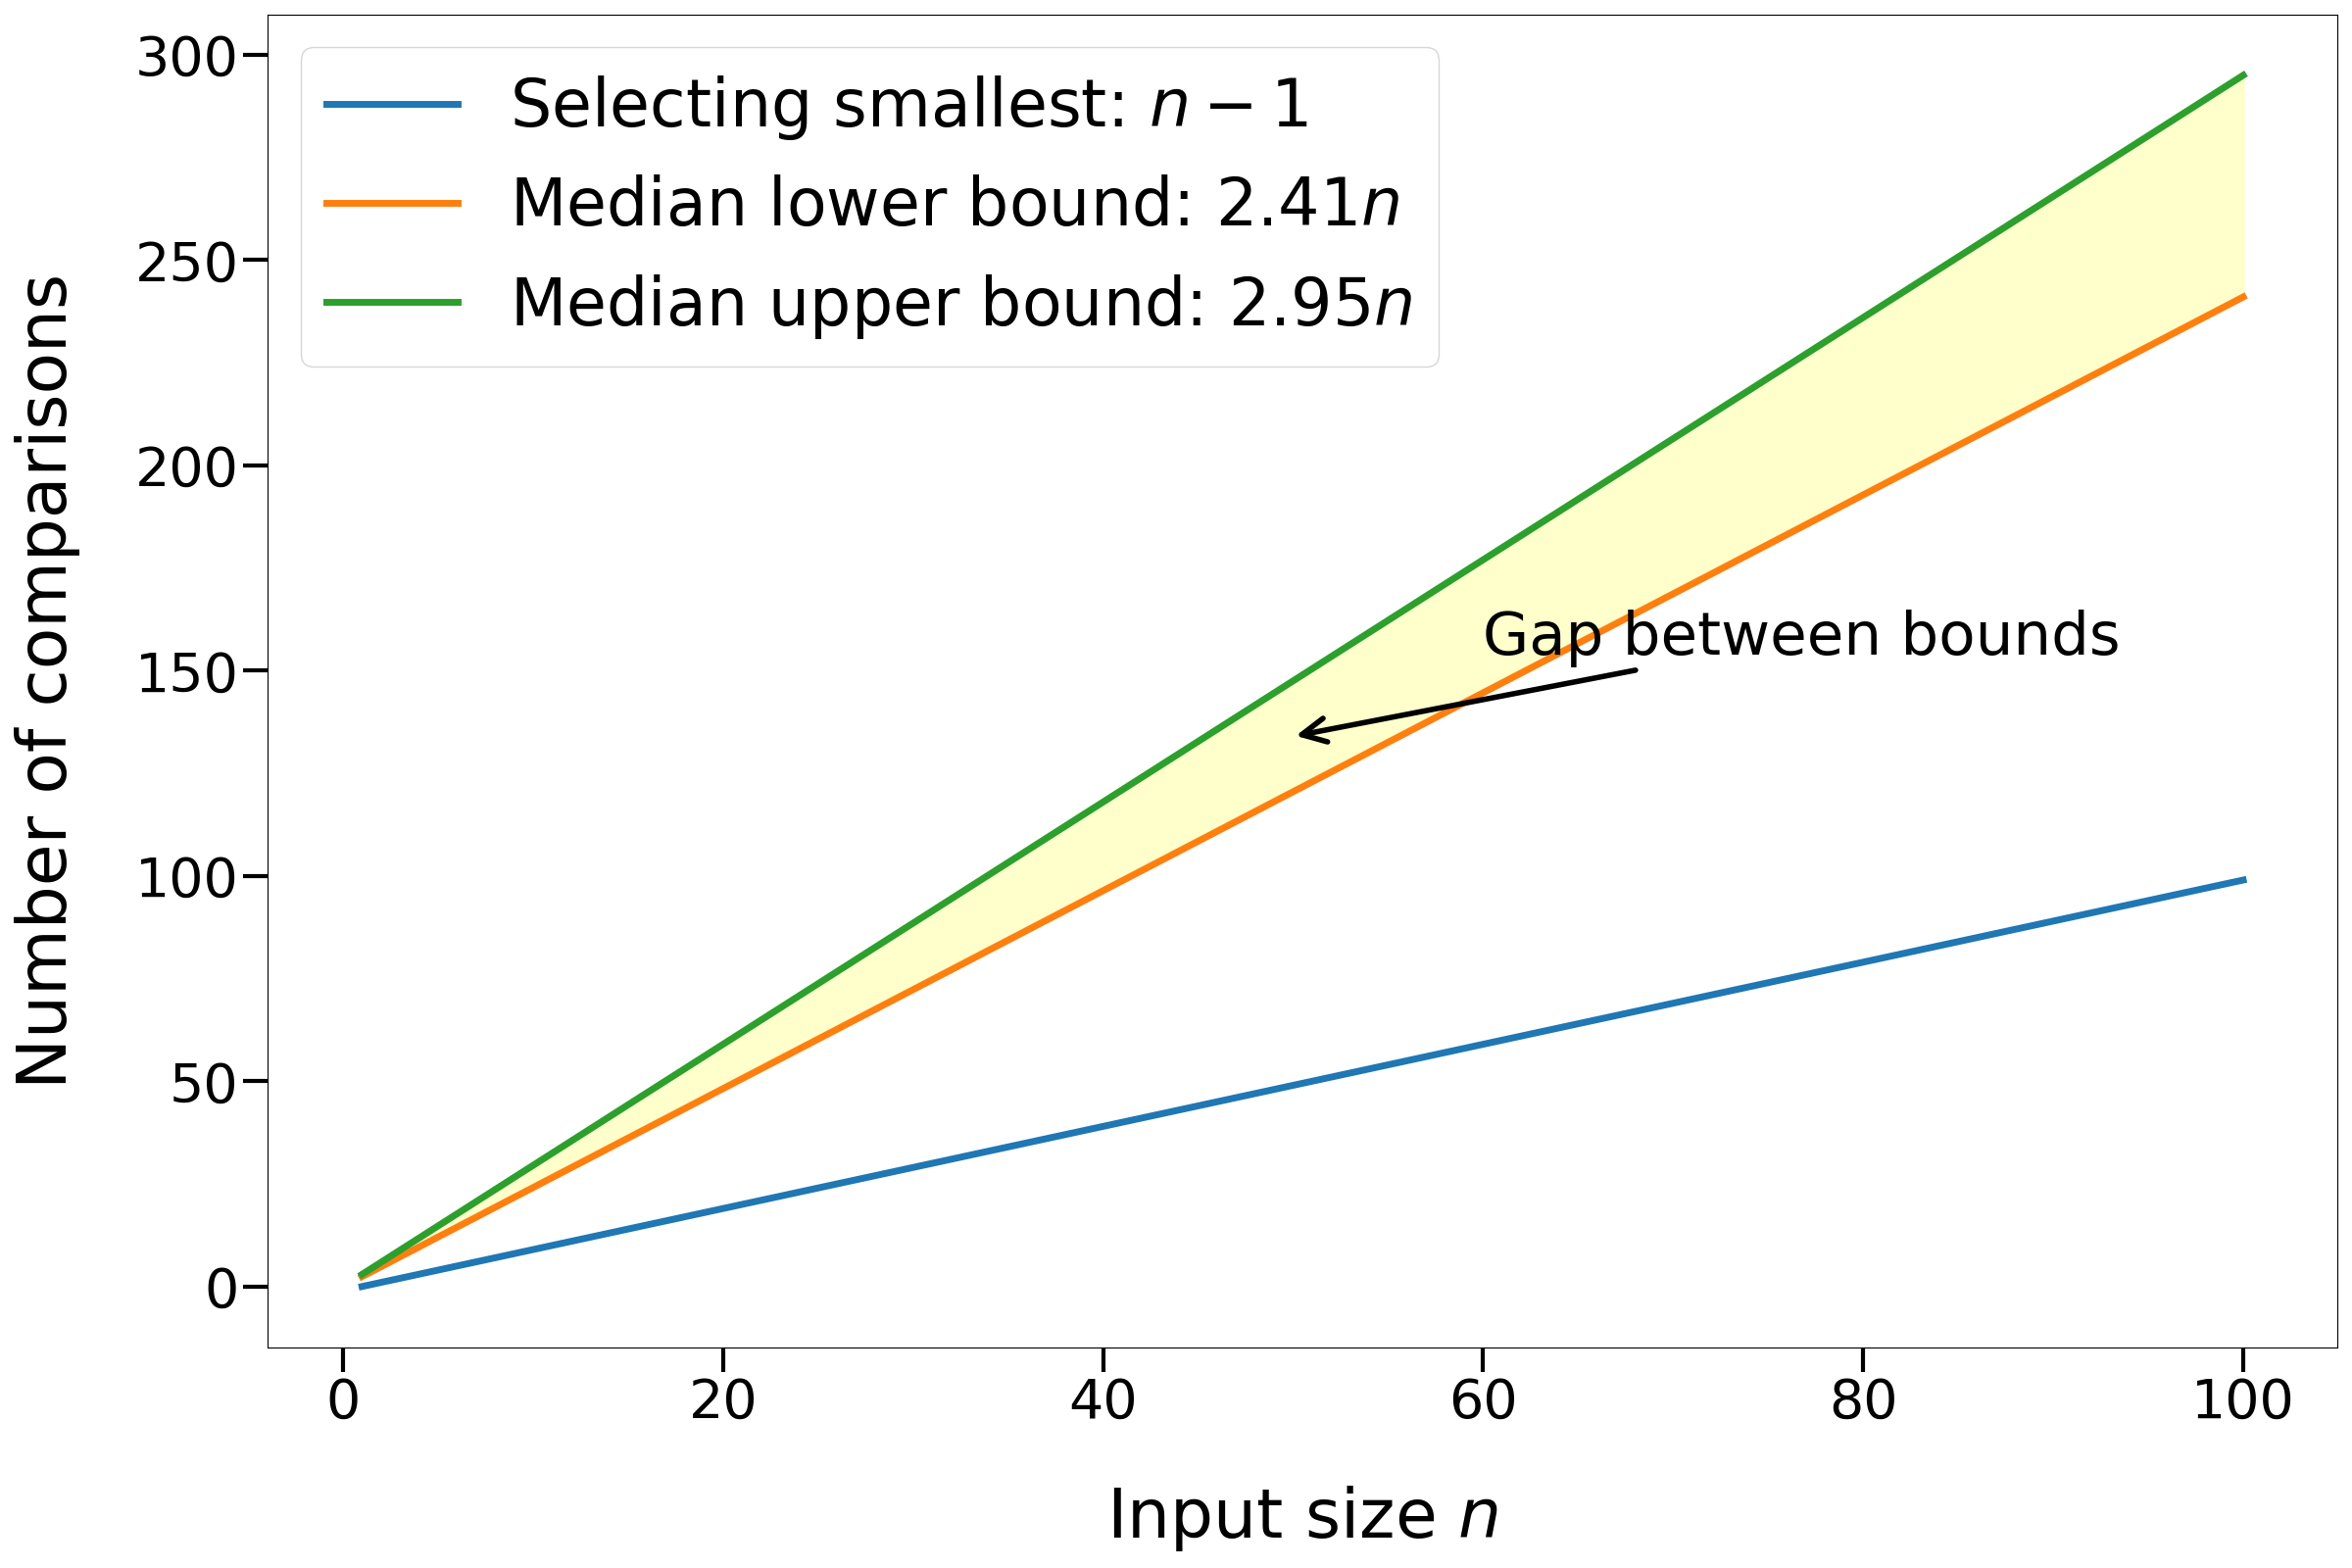
\includegraphics[height=0.5\textheight]{figures/bounds_diagram.png}
    \caption{\scriptsize Complexity Bounds for the Selection Problem}
  \end{figure}
  \textbf{Our Question:} What are the \textit{exact} values of $V_i^n$ for small $n$ and arbitrary $i$, and how do they compare to these general bounds?
  \note{
    \begin{itemize}
      \item This is summarized by the question 
      \item What are the \textit{exact} values of $V_i^n$ for small $n$ and arbitrary $i$, and how do they compare to these general bounds?
      \item Asymptotic analysis, e.g. give a good idea of the growth behavior of a problem. 
      \item However, we are intereseted in exact values for certain $n$ and $i$. A viable method to find optimal values in the worst case is Computer Search.
      \item This brings us to the previous work on this topic.
    \end{itemize}
  }
\end{frame}

\begin{frame}{Previous Work on Exact Bounds}
  \begin{tabular}{|p{6cm}|p{6cm}|}
    \hline
    \multicolumn{1}{|c|}{Gasarch, Kelly and Puth (1996)}                                               & \multicolumn{1}{c|}{Oksanen (2002)} \\
    \cline{1-2}
    \raggedright \begin{itemize}
                   \item [...]were the first to apply computer search to find lower bounds for the selection problem.
                         %\item [...]nutzten für größere $n,i$ sog. \textit{pair-forming algorithms}
                 \end{itemize} &
    \begin{itemize}
      \item[...] published a computer search algorithm that surpassed the lower bounds of Gasarch et al.
    \end{itemize}                                        \\
    \cline{1-2}
  \end{tabular}

  \note{This is a note}
\end{frame}

% \section{Grundlagen}

% \subsection{Partial Order Sets}

% \sectionframe{\insertsection}

% \begin{frame}{Zentrale Datenstruktur: Poset}
%   \textbf{Definition:}
%   \vspace{1mm}
%   \begin{itemize}
%     \item Sei $\Omega$ eine Menge mit paarweise verschiedenen Elementen mit $\vert \Omega \vert = n$.
%     \item $(n,i,R)$ bezeichnet eine Instanz des \textit{Selection}-Problems.
%     \item $R \subseteq \Omega^2$ mit $(a,b) \in R \Leftrightarrow a \leq b$.
%   \end{itemize}
%   \vspace{2mm}
% \end{frame}

% \begin{frame}{Zentrale Datenstruktur: Poset}
%   \textbf{Dualität:} \\
%   \vspace{1mm}
%   Das Duale eines Posets $P = (n, i, R)$ ist das Poset $P^{-1} = \left(n, n-1-i, R'\right)$ mit $R' = \{ (u,v) \; \vert \; (v,u) \in R\}$.

%   \pause
%   \vspace{2mm}
%   \textbf{Reduktion:} \\
%   \vspace{1mm}
%   Ein Poset heißt \textit{reduziert}, wenn es zu jedem Element höchstens $i$ viele kleinere Elemente gibt und höchstens $n-1-i$ viele größere Elemente.
% \end{frame}

% \begin{frame}{Zentrale Datenstruktur: Poset}
%   \textbf{Kanonische Form:} \\
%   \vspace{1mm}
%   Ein Poset heißt \textit{kanonifiziert}, wenn alle Elemente des Posets kanonisch angeordnet sind. Das heißt, dass alle möglichen Permutationen der Elemente auf das Poset abbilden.

%   \pause
%   \vspace{2mm}
%   \textbf{Normalform:} \\
%   \vspace{1mm}
%   Ein reduziertes und kanonifiziertes Poset heißt \textit{normalisiert}.

%   \pause
%   \vspace{2mm}
%   \textbf{Optimale Kosten:} \\
%   \vspace{1mm}
%   \textit{Kosten eines Posets} $V(P)$ mit $P=(n,i,R)$ sind die optimale Anzahl an weiteren Vergleichen, die benötigt werden, um das $i$ kleinste Element zu bestimmen.
% \end{frame}

% \begin{frame}{Ein Lemma}
%   \textbf{Lemma 1:} Für ein Poset $P=(n,i,R)$ gilt $V(P) = V(P^{-1})$.
%   \vspace{1mm}

%   \textit{Beweis: Die Berechnung von $V(P)$ ergibt gleichzeitig einen Algorithmus, der in einen Entscheidungsbaum übersetzt werden kann. Vertausche alle Kinder, und derselbe Algorithmus führt auf die Lösung von $P^{-1}$.}

% \end{frame}

% \begin{frame}{Ein Beispiel mit Poset-Reduktion}
%   \begin{figure}
%     \begin{tikzpicture}[tcancel/.append style={draw=#1, cross out, inner sep=6pt}]
  \draw(-.5, -.5) rectangle (4.5, .5);
  \node[circle,draw=black] (A1) at (0, 0) {};
  \node[circle,draw=black] (A2) at (1, 0) {};
  \node[circle,draw=black] (A3) at (2, 0) {};
  \node[circle,draw=black] (A4) at (3, 0) {};
  \node[circle,draw=black] (A5) at (4, 0) {};

  \draw[dashed] (A1) -- (A2) node {};
  \draw[dashed] (A3) -- (A4) node {};

  \draw(-0.5, -2.6) rectangle (4.5, -0.8);
  \node[circle,draw=black] (B1) at (1.0, 0 - 2.2) {};
  \node[circle,draw=black] (B2) at (1.0, 1 - 2.2) {};
  \node[circle,draw=black] (B3) at (2.0, 0 - 2.2) {};
  \node[circle,draw=black] (B4) at (2.0, 1 - 2.2) {};
  \node[circle,draw=black] (B5) at (4.0, 0.5 - 2.2) {};

  \draw (B1) -- (B2) node {};
  \draw (B3) -- (B4) node {};
  \draw[dashed] (B2) -- (B4) node {};

  \draw(-0.5, -5.5) rectangle (4.5, -2.9);
  \node[circle,draw=black] (C1) at (1, 0 - 5.0) {};
  \node[circle,draw=black] (C2) at (1, 1 - 5.0) {};
  \node[circle,draw=black,tcancel=red] (C3) at (2, 1.5 - 5.0) {};
  \node[circle,draw=black] (C3) at (2, 1.5 - 5.0) {};
  \node[circle,draw=black] (C4) at (2, .5 - 5.0) {};
  \node[circle,draw=black] (C5) at (3, .5 - 5.0) {};

  \draw (C1) -- (C2) node {};
  \draw (C3) -- (C4) node {};
  \draw (C2) -- (C3) node {};
  \draw[dashed] (C4) -- (C5) node {};

  \draw(5.5, -1.3) rectangle (10.5, .5);
  \node[circle,draw=black] (D1) at (6, 0.1 - 1) {};
  \node[circle,draw=black] (D2) at (6, 0.1) {};
  \node[circle,draw=black] (D3) at (7, 0.1 - 1) {};
  \node[circle,draw=black] (D4) at (7, 0.1 ) {};
  \node[circle,draw=black,tcancel=red] (D5) at (10.0, 0.1 -0.5) {};
  \node[circle,draw=black] (D5) at (10.0, 0.1 -0.5) {};

  \draw (D1) -- (D2) node {};
  \draw (D3) -- (D4) node {};
  \draw[dashed] (D2) -- (D4) node {};

  \draw(5.5, -4.1) rectangle (10.5, -1.6);
  \node[circle,draw=black,tcancel=red] (E1) at (8, 1.5 - 3.6) {};
  \node[circle,draw=black] (E1) at (8, 1.5 - 3.6) {};

  \node[circle,draw=black] (E2) at (7, 1 - 3.6) {};
  \node[circle,draw=black,tcancel=red] (E3) at (7, 0 - 3.6) {};
  \node[circle,draw=black] (E3) at (7 , 0 - 3.6) {};

  \node[circle,draw=black] (E4) at (8, 0.5 - 3.6) {};

  \node[circle,draw=black,tcancel=red] (E5) at (9, 0.5 - 3.6) {};
  \node[circle,draw=black] (E5) at (9, 0.5 - 3.6) {};

  \draw (E1) -- (E2) node {};
  \draw (E1) -- (E4) node {};
  \draw (E2) -- (E3) node {};
  \draw[dashed] (E2) -- (E4) node {};

\end{tikzpicture}
%   \end{figure}

% \end{frame}

% \subsection{Kompatible Lösungen}
% \begin{frame}{\insertsubsection}
%   \centering
%   \begin{tikzpicture}

%     \node[draw, circle] (l0) at (0, 0) {};
%     \node[draw, circle] (l1) at (1, 0) {};
%     \node[draw, circle] (l2) at (2, 0) {};
%     \node[draw, circle] (l3) at (3, 0) {};

%     \node[draw, circle] (I) at (1.5, 2) {$i$};

%     \path[draw] (l0) to (I);
%     \path[draw] (l1) to (I);
%     \path[draw] (l2) to (I);
%     \path[draw] (l3) to (I);

%     \node[draw, circle] (u0) at (0.5, 4) {};
%     \node[draw, circle] (u1) at (1.5, 4) {};
%     \node[draw, circle] (u2) at (2.5, 4) {};

%     \path[draw] (u0) to (I);
%     \path[draw] (u1) to (I);
%     \path[draw] (u2) to (I);

%   \end{tikzpicture}

% \end{frame}

% \begin{frame}{\insertsubsection}
%   \centering
%   \begin{tikzpicture}

%     \node[draw, circle] (fl0) at (0, 0) {};
%     \node[draw, circle] (fl1) at (1, 0) {};
%     \node[draw, circle] (fl2) at (2, 0) {};
%     \node[draw, circle] (fl3) at (3, 0) {};

%     \node[draw, circle] (fI) at (1.5, 2) {$i$};

%     \path[draw] (fl0) to (fI);
%     \path[draw] (fl1) to (fI);
%     \path[draw] (fl2) to (fI);
%     \path[draw] (fl3) to (fI);

%     \node[draw, circle] (fu0) at (0.5, 4) {};
%     \node[draw, circle] (fu1) at (1.5, 4) {};
%     \node[draw, circle] (fu2) at (2.5, 4) {};

%     \path[draw] (fu0) to (fI);
%     \path[draw] (fu1) to (fI);
%     \path[draw] (fu2) to (fI);

%     \path[draw=red] (fu0) to (fl1);

%     %second

%     \node[draw, circle] (sl0) at (0 + 5, 0) {};
%     \node[draw, circle] (sl1) at (1 + 5, 0) {};
%     \node[draw, circle] (sl2) at (2 + 5, 0) {};
%     \node[draw, circle] (sl3) at (3 + 5, 0) {};

%     \node[draw, circle] (sI) at (1.5 + 5, 2) {$i$};

%     \path[draw] (sl0) to (sI);
%     \path[draw] (sl1) to (sI);
%     \path[draw] (sl2) to (sI);
%     \path[draw] (sl3) to (sI);

%     \node[draw, circle] (su0) at (0.5 + 5, 4) {};
%     \node[draw, circle] (su1) at (1.5 + 5, 4) {};
%     \node[draw, circle] (su2) at (2.5 + 5, 4) {};

%     \path[draw] (su0) to (sI);
%     \path[draw] (su1) to (sI);
%     \path[draw] (su2) to (sI);

%     \path[draw=red] (su0) to (su1);

%   \end{tikzpicture}

% \end{frame}

% \subsection{Kompatible Lösungen}
% \begin{frame}{\insertsubsection}
%   \centering
%   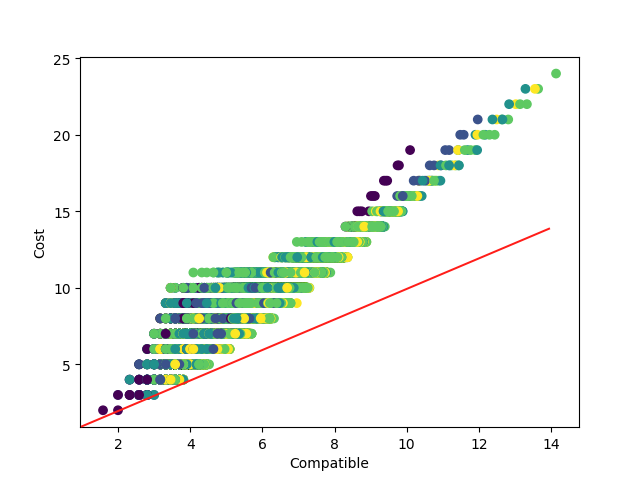
\includegraphics[scale=.5]{../article/figures/compatible_cost_relation.png}

% \end{frame}




\section{Forward Search}
\sectionframe{\insertsection}

\begin{frame}{\insertsection: A Minimax Approach}
  \centering
  \begin{tikzpicture}
    [
      level 1/.style = {sibling distance = 4cm},
      level 2/.style = {sibling distance = 2.5cm},
    ]

    \node[anchor=east] at (-7,0) {Min};
    \node[anchor=east] at (-7,-1.5) {Max};
    \node[anchor=east] at (-7,-3) {Min};
    \node[anchor=east] at (-7,-4.5) {Max};

    \node[] (root) {$(n,i,\emptyset)$}
    child {
        node[] {$\{a,b\}$}
        child {
            node[] {$(n,i,\{(a,b)\})$}
            child[sibling distance = 1cm] {
                node[] {$\{c,d\}$}
                child[sibling distance = 1cm] { node[] {$\cdots$}}
                child[sibling distance = 1cm] { node[] {$\cdots$}}
              }
            child[sibling distance = 1cm] { node[] {$\cdots$}}
          }
        child {
            node[] {$(n,i,\{(b,a)\})$}
            child[sibling distance = 1cm] {
                node[] {$\{c,d\}$}
                child[sibling distance = 1cm] { node[] {$\cdots$}}
                child[sibling distance = 1cm] { node[] {$\cdots$}}
              }
            child[sibling distance = 1cm] { node[] {$\cdots$}}
          }
      }
    child {
        node {$\{a,c\}$}
        child[sibling distance = 1cm] { node[] {$\cdots$}}
        child[sibling distance = 1cm] { node[] {$\cdots$}}
      }
    child {
        node[] {$\cdots$}
      }
    ;

  \end{tikzpicture}
  \note{
    \begin{itemize}
      \item The forward search starts with the empty poset and recursively determines the cost of selecting the $i$-th smallest element of a poset $P$.
      \item This is implemented using a minimax algorithm.
      \item Between all pairs of elements the pair is compared that yields the smallest number of comparisons.
      \item Between the two possible outcomes of a comparison, the worst case is assumed.
      \item To save memory and enable pruning, the search tree is traversed using a depth-first search.
      \item The maximum number of comparisons assigned to child problems is limited to one less than the current best result.
      \item The search program builds algorithms by recording, for each problem, the comparison that led to the cheapest result.
    \end{itemize} }
\end{frame}

\begin{frame}{Optimizations}
  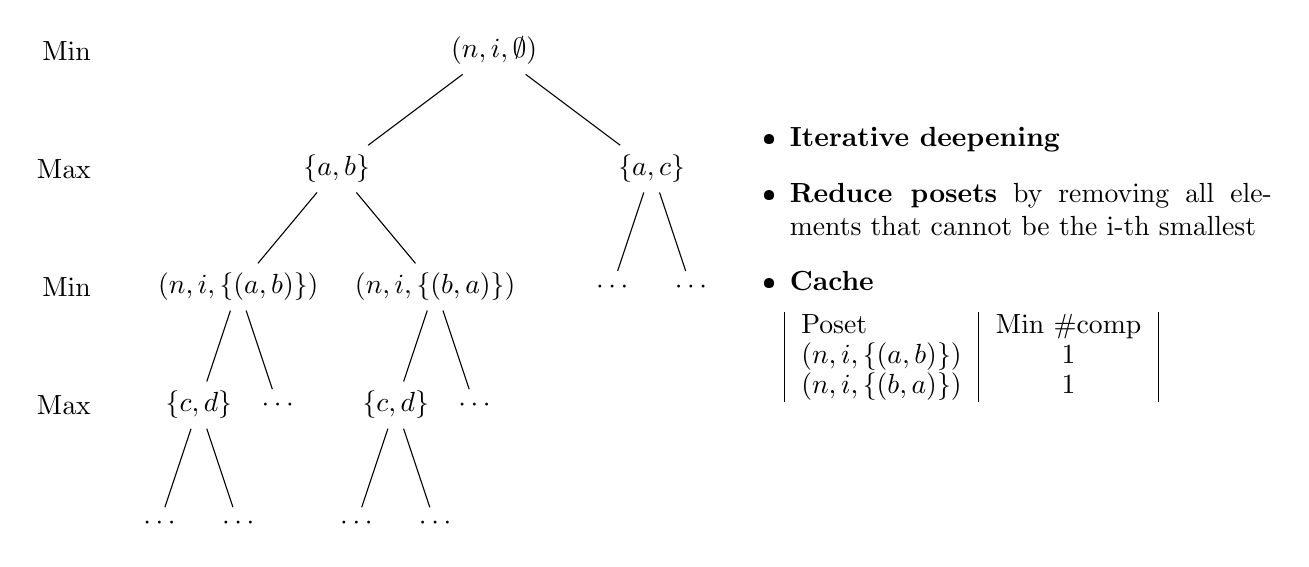
\begin{tikzpicture}
    [
      level 1/.style = {sibling distance = 4cm},
      level 2/.style = {sibling distance = 2.5cm},
    ]

    \node[anchor=east] at (-12,2) {Min};
    \node[anchor=east] at (-12,0.5) {Max};
    \node[anchor=east] at (-12,-1) {Min};
    \node[anchor=east] at (-12,-2.5) {Max};

    \node[] (root) at (-7,2) {$(n,i,\emptyset)$}
    child {
        node[] {$\{a,b\}$}
        child {
            node[] {$(n,i,\{(a,b)\})$}
            child[sibling distance = 1cm] {
                node[] {$\{c,d\}$}
                child[sibling distance = 1cm] { node[] {$\cdots$}}
                child[sibling distance = 1cm] { node[] {$\cdots$}}
              }
            child[sibling distance = 1cm] { node[] {$\cdots$}}
          }
        child {
            node[] {$(n,i,\{(b,a)\})$}
            child[sibling distance = 1cm] {
                node[] {$\{c,d\}$}
                child[sibling distance = 1cm] { node[] {$\cdots$}}
                child[sibling distance = 1cm] { node[] {$\cdots$}}
              }
            child[sibling distance = 1cm] { node[] {$\cdots$}}
          }
      }
    child {
        node {$\{a,c\}$}
        child[sibling distance = 1cm] { node[] {$\cdots$}}
        child[sibling distance = 1cm] { node[] {$\cdots$}}
      };

    \node[anchor=north east] at (3, 1.5) {
      \parbox{7cm}{
        \begin{itemize}
          \item \textbf{Iterative deepening}
          \item \textbf{Reduce posets} by removing all elements that cannot be the i-th smallest
          \item \textbf{Cache}
        \end{itemize}
      }
    };
    \node[anchor=north east] at (1.8,-1.2) {
      \parbox{5cm}{
        \begin{tabular}{|l|c|}
          \toprule
          Poset             & Min \#comp \\
          \midrule
          $(n,i,\{(a,b)\})$ & 1          \\
          $(n,i,\{(b,a)\})$ & 1          \\
          \bottomrule
        \end{tabular}
      }
    };
  \end{tikzpicture}

  \note{\begin{itemize}
      \item We apply depth-first search with iterative deepening.
      \item This saves memory and previous results are cached.
      \item We work on reduced posets. For each poset we remove elements that cannot be the i-th smallest. So if an element has more than $i-1$ elements that are smaller, or more than $n-i$ elements that are larger, it is removed from the poset.
      \item We store an approximated canonical representation of the problem and its dual in the cache along with the number of comparisons applied so far.
      \item Each entry indicates that the poset is not solvable with just this amount of comparisons.
      \item Besides for simple reusing purposes, the information in the chach can be used for pruning, by cutting off branches that contradict the minimum value in the cache.
    \end{itemize}
  }
\end{frame}

\begin{frame}{Pruning techniques}
  \begin{itemize}
    \item Compatible Solutions
    \item Free Comparison
  \end{itemize}

  \note{\begin{itemize}
      \item We applied to furhter pruning techniques, which are based on compatible solutions and a free comparison
    \end{itemize}
  }
\end{frame}

\begin{frame}{Pruning technique: Compatible solutions}

  The solved problem $(S,i)$ is a \textbf{compatible solution} of the problem $(R,i)$, if
  \begin{align*}
    a \leq_S b \Rightarrow b \not \leq a
  \end{align*}
  \vspace{1mm}

  Denote the \textbf{number of compatible solutions} with $\vert \mathcal{C}(P,i) \vert $\\
  \vspace{5mm}
  \hspace{-3mm}
  \begin{tabular}{l p{8cm}}
    \textbf{Lemma: } & Selecting the i-th smallest element of a poset P requires at least $\lceil log (|C(P, i)|) \rceil $ comparisons
  \end{tabular}
\end{frame}

\begin{frame}{Pruning technique: Compatible solutions}
  \only<1>{
    \begin{tikzpicture}
      [
        level 1/.style = {sibling distance = 4cm},
        level 2/.style = {sibling distance = 2.5cm},
      ]

      \node[anchor=east] at (-7,0) {Min};
      \node[anchor=east] at (-7,-1.5) {Max};
      \node[anchor=east] at (-7,-3) {Min};
      \node[anchor=east] at (-7,-4.5) {Max};

      \node[] (root) {$(n,i,\emptyset)$}
      child {
          node[] {$\{a,b\}$}
          child {
              node[] {$(n,i,\{(a,b)\})$}
              child[sibling distance = 1cm] {
                  node[] {$\{c,d\}$}
                  child[sibling distance = 1cm] { node[] {$\cdots$}}
                  child[sibling distance = 1cm] { node[] {$\cdots$}}
                }
              child[sibling distance = 1cm] { node[] {$\cdots$}}
            }
          child {
              node[] {$(n,i,\{(b,a)\})$}
              child[sibling distance = 1cm] {
                  node[] {\color{black}$\{c,d\}$}
                  child[sibling distance = 1cm, edge from parent/.style={draw,dashed}] { node[] {\color{red}42}}
                  child[sibling distance = 1cm] { node[] {$\cdots$}}
                }
              child[sibling distance = 1cm] { node[] {$\cdots$}}
            }
        }
      child {
          node {$\cdots$}
        }
      child {
          node[] {$\cdots$}
        }
      ;

    \end{tikzpicture}
  }
  \only<2>{
    \begin{tikzpicture}
      [
        level 1/.style = {sibling distance = 4cm},
        level 2/.style = {sibling distance = 2.5cm},
      ]

      \node[anchor=east] at (-7,0) {Min};
      \node[anchor=east] at (-7,-1.5) {Max};
      \node[anchor=east] at (-7,-3) {Min};
      \node[anchor=east] at (-7,-4.5) {Max};

      \node[] (root) {$(n,i,\emptyset)$}
      child {
          node[] {$\{a,b\}$}
          child {
              node[] {$(n,i,\{(a,b)\})$}
              child[sibling distance = 1cm] {
                  node[] {$\{c,d\}$}
                  child[sibling distance = 1cm] { node[] {$\cdots$}}
                  child[sibling distance = 1cm] { node[] {$\cdots$}}
                }
              child[sibling distance = 1cm] { node[] {$\cdots$}}
            }
          child {
              node[] {$(n,i,\{(b,a)\})$}
              child[sibling distance = 1cm,red] {
                  node[] {\color{black}$\{c,d\}$}
                  child[sibling distance = 1cm,red, edge from parent/.style={draw,dashed}] { node[] {\color{red}42}}
                  child[sibling distance = 1cm,black] { node[] {$\cdots$}}
                }
              child[sibling distance = 1cm] { node[] {$\cdots$}}
            }
        }
      child {
          node {$\cdots$}
        }
      child {
          node[] {$\cdots$}
        }
      ;

      \node [draw=none] at (-1, -3) {\color{red} $(\_, 42)$};
    \end{tikzpicture}
  }
  \only<3>{
    \begin{tikzpicture}
      [
        level 1/.style = {sibling distance = 4cm},
        level 2/.style = {sibling distance = 2.5cm},
      ]

      \node[anchor=east] at (-7,0) {Min};
      \node[anchor=east] at (-7,-1.5) {Max};
      \node[anchor=east] at (-7,-3) {Min};
      \node[anchor=east] at (-7,-4.5) {Max};

      \node[] (root) {$(n,i,\emptyset)$}
      child {
          node[] {$\{a,b\}$}
          child {
              node[] {$(n,i,\{(a,b)\})$}
              child[sibling distance = 1cm] {
                  node[] {$\{c,d\}$}
                  child[sibling distance = 1cm] { node[] {$\cdots$}}
                  child[sibling distance = 1cm] { node[] {$\cdots$}}
                }
              child[sibling distance = 1cm] { node[] {$\cdots$}}
            }
          child {
              node[] {$(n,i,\{(b,a)\})$}
              child[sibling distance = 1cm,red] {
                  node[] {\color{black}$\{c,d\}$}
                  child[sibling distance = 1cm,red,, edge from parent/.style={draw,dashed}] { node[] {\color{red}42}}
                  child[sibling distance = 1cm,black] { node[] {$\cdots$}}
                }
              child[sibling distance = 1cm] { node[] {$\cdots$}}
            }
        }
      child {
          node {$\cdots$}
        }
      child {
          node[] {$\cdots$}
        }
      ;

      \draw[red] (-3.7,-2) -- (-3,-2.5);
      \draw[red] (-3.7,-2.5) -- (-3,-2);

      \node [draw=none] at (-1, -3) {\color{red} $(\_, 42)$};
      \node [draw=none] at (-1, -2.25) {\color{red} If $42 < \lceil \log (\vert \mathcal{C}(P,i)\vert ) \rceil$};


    \end{tikzpicture}
  }

  \note{
    \begin{itemize}
      \item For example when one child turns out to be solvable with 42 comparisons, the value is propagated upwards. And e.g. this is a min node so upon completion the solution is at most 42. But when log of number of compatible solutions is larger than 42 this branch can be pruned.
    \end{itemize}
  }
\end{frame}

\begin{frame}{Pruning technique: Free comparison}
  \begin{columns}
    \begin{column}{0.65\textwidth}
      \begin{itemize}
      \item Already applied by Oksanen
      \item Idea: Add a useful relation between a large element and a small element
      \item Search for unrelated elements $a$ and $b$ such that a has at least two elements less than it and b has at least two elements greater than it
    \end{itemize}
    \end{column}
    \begin{column}{0.35\textwidth}
      \begin{figure}
        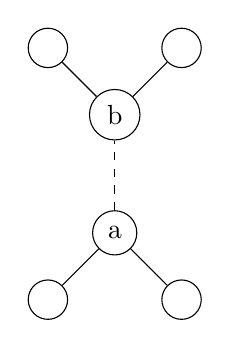
\begin{tikzpicture}[node distance=1.2cm]
          \node[draw, circle, minimum size=0.5cm] (1) {a};
          \node[draw, circle, minimum size=0.5cm, below right of=1] (2) {};
          \node[draw, circle, minimum size=0.5cm, below left of=1] (3) {};

          \node[draw, circle, minimum size=0.5cm, above of=1, node distance=1.5cm] (4) {b};
          \node[draw, circle, minimum size=0.5cm, above right of=4] (5) {};
          \node[draw, circle, minimum size=0.5cm, above left of=4] (6) {};
          
          \path[dashed] (1) edge (4);
          
          \path[-]
          (1) edge (2)
          (1) edge (3)
          (4) edge (5)
          (4) edge (6);
        \end{tikzpicture}
      \end{figure}
    \end{column}
    \end{columns}
\end{frame}

\author{SEA 2025 \hspace{1cm} Julius von Smercek}

\section{Backward Search}
\sectionframe{\insertsection}

\begin{frame}{\insertsection}
  Start with a solved poset and search the empty poset
  \vfill
  \begin{itemize}
    \item<+-> \textbf{Goal:} Given an upper bound $k$, find all posets solvable in at most $k$ comparisons.
    \item<+-> \textbf{Initialization:} Start with the set of all posets that are already ``solved'' (i.e., the $i$-th element is uniquely identified). Their cost is 0.
    \item<+-> \textbf{Iteration (Level $k \to k+1$):} To find all posets solvable in $k+1$ steps, find all \textit{predecessors} of posets solvable in $\leq k$ steps.
    \item<+-> \textbf{Termination:} The search stops when the initial empty poset $(n, i, \emptyset)$ is generated. Its level is the value $V_i^n$.
    \item<+-> \textbf{Canonization:} A unique normal form (with `nauty`) is expensive, but required. We use fast invariants to pre-filter, such that `nauty` is needed for only $< 0.1\%$ of posets.
  \end{itemize}
\end{frame}

\begin{frame}{Predecessor Computation}
  \begin{definition}[Predecessor]
    Suppose the set of all posets solvable in $k$ comparisons is known.
    A normalized poset $Q$ is a \textbf{predecessor} iff there exists a comparison between two elements $u,v$ such that
    \begin{enumerate}
      \item<+-> Adding the relation $(u,v)$ to $Q$ yields a known poset solvable in exact $k$ steps
      \item<+-> Adding the relation $(v,u)$ to $Q$ yields a known poset solvable in at maximum $k$ steps
      \item<+-> $Q$ itself was not found at a lower level
    \end{enumerate}
  \end{definition}
  \vfill
  This process essentially ``removes'' a comparison to go one step backward.
\end{frame}

\begin{frame}{Example}
  \vspace{-0.75cm}
  \begin{figure}[!b]
    \centering
    \scalebox{0.8}{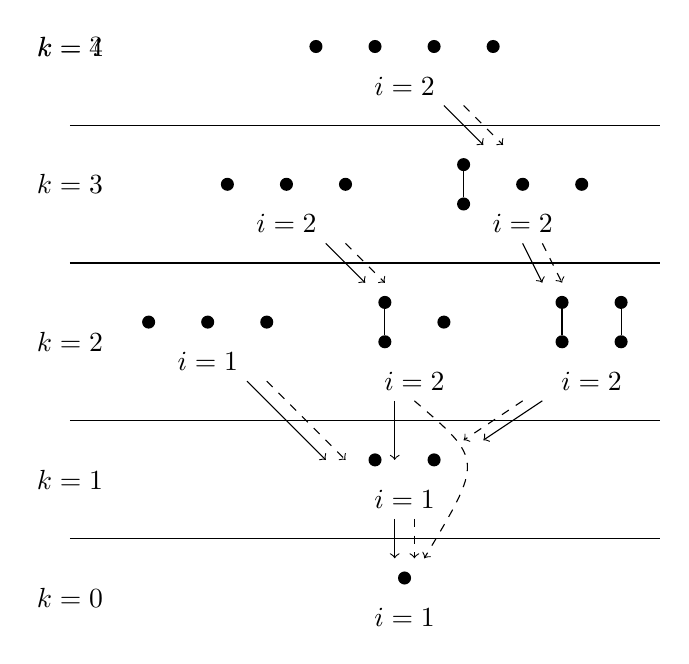
\begin{tikzpicture}

  % Level k = 4
  \uncover<1-3>{
    \node at (-1, 8) {$k=\text{ ?}$};
  }
  \uncover<4->{
    \node at (-1, 8) {$k=4$};
  }

  \node[circle,fill=black,scale=0.5] (k4_1) at (2.125 + 0 * 0.75, 8) {};
  \node[circle,fill=black,scale=0.5] (k4_2) at (2.125 + 1 * 0.75, 8) {};
  \node[circle,fill=black,scale=0.5] (k4_3) at (2.125 + 2 * 0.75, 8) {};
  \node[circle,fill=black,scale=0.5] (k4_4) at (2.125 + 3 * 0.75, 8) {};
  \node at (2.125 + 0.75 * 1.5, 7.5) {$i=2$};

  \uncover<4->{
    \draw[->, dashed] (4, 7.25) -- (4.5, 6.75);
    \draw[->] (3.75, 7.25) -- (4.25, 6.75);

    \draw (-1, 7) -- (6.5, 7);

    % Level k = 3
    \node at (-1, 6.25) {$k=3$};

    \node[circle,fill=black,scale=0.5] (k3_1) at (1 + 0 * 0.75, 6.25) {};
    \node[circle,fill=black,scale=0.5] (k3_2) at (1 + 1 * 0.75, 6.25) {};
    \node[circle,fill=black,scale=0.5] (k3_3) at (1 + 2 * 0.75, 6.25) {};
    \node at (1 + 0.75, 5.75) {$i=2$};

    \draw[->, dashed] (2.5, 5.5) -- (3, 5);
    \draw[->] (2.25, 5.5) -- (2.75, 5);

    \node[circle,fill=black,scale=0.5] (k3_4) at (4 + 0 * 0.75, 6.5) {};
    \node[circle,fill=black,scale=0.5] (k3_5) at (4 + 0 * 0.75, 6) {};
    \node[circle,fill=black,scale=0.5] (k3_6) at (4 + 1 * 0.75, 6.25) {};
    \node[circle,fill=black,scale=0.5] (k3_7) at (4 + 2 * 0.75, 6.25) {};
    \draw (k3_4) -- (k3_5);
    \node at (4 + 0.75, 5.75) {$i=2$};

    \draw[->, dashed] (5, 5.5) -- (5.25, 5);
    \draw[->] (4.75, 5.5) -- (5, 5);
  } \uncover<3->{

    \draw (-1, 5.25) -- (6.5, 5.25);

    % Level k = 2
    \node at (-1, 4.25) {$k=2$};

    \node[circle,fill=black,scale=0.5] (k2_1) at (0 + 0 * 0.75, 4.5) {};
    \node[circle,fill=black,scale=0.5] (k2_2) at (0 + 1 * 0.75, 4.5) {};
    \node[circle,fill=black,scale=0.5] (k2_3) at (0 + 2 * 0.75, 4.5) {};
    \node at (0 + 0.75, 4) {$i=1$};

    \draw[->, dashed] (1.5, 3.75) -- (2.5, 2.75);
    \draw[->] (1.25, 3.75) -- (2.25, 2.75);

    \node[circle,fill=black,scale=0.5] (k2_4) at (3 + 0 * 0.75, 4.25) {};
    \node[circle,fill=black,scale=0.5] (k2_5) at (3 + 0 * 0.75, 4.75) {};
    \node[circle,fill=black,scale=0.5] (k2_6) at (3 + 1 * 0.75, 4.5) {};
    \draw (k2_4) -- (k2_5);
    \node at (3 + 0.75 * 0.5, 3.75) {$i=2$};

    \draw[->, dashed] (3.375, 3.5) .. controls (4.25, 2.75) .. (3.5, 1.5);
    \draw[->] (3.125, 3.5) -- (3.125, 2.75);

    \node[circle,fill=black,scale=0.5] (k2_7) at (5.25 + 0 * 0.75, 4.25) {};
    \node[circle,fill=black,scale=0.5] (k2_8) at (5.25 + 0 * 0.75, 4.75) {};
    \node[circle,fill=black,scale=0.5] (k2_9) at (5.25 + 1 * 0.75, 4.25) {};
    \node[circle,fill=black,scale=0.5] (k2_10) at (5.25 + 1 * 0.75, 4.75) {};
    \draw (k2_7) -- (k2_8);
    \draw (k2_9) -- (k2_10);
    \node at (5.25 + 0.75 * 0.5, 3.75) {$i=2$};

    \draw[->, dashed] (4.75, 3.5) -- (4, 3);
    \draw[->] (5, 3.5) -- (4.25, 3);
  } \uncover<2->{

    \draw (-1, 3.25) -- (6.5, 3.25);
    % Level k = 1
    \node at (-1, 2.5) {$k=1$};

    \node[circle,fill=black,scale=0.5] (k1_1) at (2.875 + 0 * 0.75, 2.75) {};
    \node[circle,fill=black,scale=0.5] (k1_2) at (2.875 + 1 * 0.75, 2.75) {};
    \node at (2.875 + 0.75 * 0.5, 2.25) {$i=1$};

    \draw[->, dashed] (3.375, 2) -- (3.375, 1.5);
    \draw[->] (3.125, 2) -- (3.125, 1.5);
  }

  \draw (-1, 1.75) -- (6.5, 1.75);

  % Level k = 0
  \node at (-1, 1) {$k=0$};

  \node[circle,fill=black,scale=0.5] (k0_1) at (3.25, 1.25) {};
  \node at (3.25, 0.75) {$i=1$};
\end{tikzpicture}
}
    \caption{Search tree for $n=4,i=2$}
    \label{fig:backward-searchtree-bound4}
  \end{figure}

  \note{
    \begin{itemize}
      \item Level k contains all posets that can be solved in k comparisons and can be formed from the previous level(s)
      \item solid arrows: point to a poset in level k - 1 that results from removing a comparison
      \item dashed arrows: point to the poset that results when the inverse comparison is added (all levels less than k)
      \item Backward search starts at the bottom at k = 0, the only ``solved'' poset
      \item compute level k + 1 as follows:
        \begin{itemize}
          \item first, try to remove a comparison
          \item add an element with comparisons such that solvability is not affected \& then remove a comparison
        \end{itemize}
    \end{itemize}
  }
\end{frame}

\begin{frame}{Removing Comparisons}
  \begin{figure}[!b]
    \centering
    \scalebox{1.5}{\begin{tikzpicture}
  \node[circle,draw=black] (A1) at (0, 0) {};
  \node[circle,draw=black] (A2) at (0, 1) {};
  \node[circle,draw=black] (A3) at (0, 2) {};

  \draw (A1) -- (A2) node {};
  \draw (A2) -- (A3) node {};
  \node (AL) at (0, -0.5) {$i = 1$};
  \node (A) at (0, -1) {(1)};


  \node[circle,draw=black] (B1) at (2.5 + 0, 0) {};
  \node[circle,draw=black] (B2) at (2.5 + 0, 2) {};
  \node[circle,draw=black] (B3) at (2.5 + 1, 1) {};

  \draw (B1) -- (B2) node {};
  \node (BL) at (2.5 + 0.5, -0.5) {$i = 1$};
  \node (B) at (2.5 + 0.5, -1) {(2)};


  \node[circle,draw=black] (C1) at (5 + 1, 2) {};
  \node[circle,draw=black] (C2) at (5 + 0, 0) {};
  \node[circle,draw=black] (C3) at (5 + 2, 0) {};

  \draw (C1) -- (C2) node {};
  \draw (C1) -- (C3) node {};
  \node (CL) at (5 + 1, -0.5) {$i = 1$};
  \node (C) at (5 + 1, -1) {(3)};
\end{tikzpicture}}
    \caption{TODO}
    \label{fig:backward-problematic-case}
  \end{figure}

  \note{
  }
\end{frame}


\begin{frame}{Multithreading}
  % 1  core : 7h 2m 59s
  % 32 cores:   20m 11s
  \vspace{-1cm}

  \begin{figure}
    \centering
    \resizebox{0.8\textheight}{!}{%
      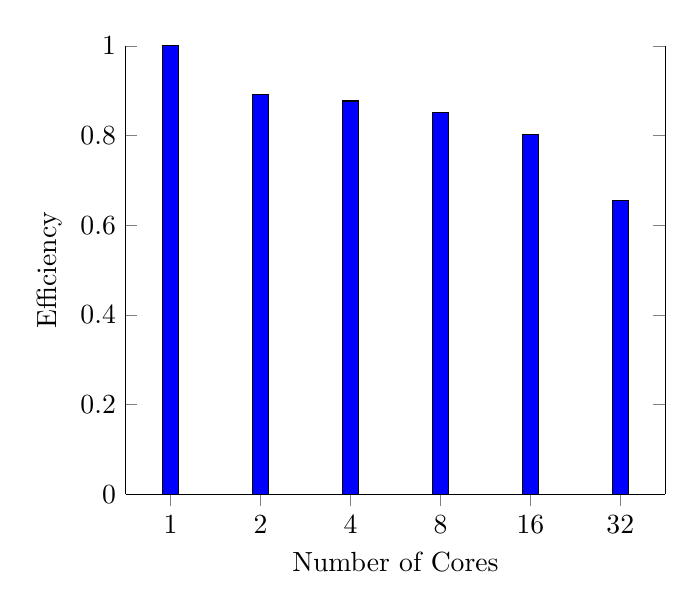
\begin{tikzpicture}
        \begin{axis}[
            ymin=0,
            ymax=1,
            axis x line=bottom,
            enlarge x limits=0.1,
            x axis line style={-},
            ylabel={Efficiency},
            xlabel={Number of Cores},
            ybar, % This makes the plot a bar chart
            bar width=0.2cm, % Adjust bar width
            % nodes near coords, % Display values on top of bars
            xtick=data, % Set x-ticks to data points
            symbolic x coords={1, 2, 4, 8, 16, 32}, % Specify the x-tick labels
          ]
          \addplot[
            ybar,
            fill=blue
          ] coordinates {
              (1, 1.000)
              (2, 0.892)
              (4, 0.877)
              (8, 0.851)
              (16, 0.803)
              (32, 0.655)
            };
        \end{axis}
      \end{tikzpicture}%
    }
    \caption{Efficiency of Parallelization for $n = 13, i = 6$}
  \end{figure}

  $\text{Efficiency} = (\text{single-core time}) \div (\text{number of cores} \cdot \text{multi-core time})$ \\
\end{frame}

\begin{frame}{Poset Distribution}
  \begin{figure}[!b]
    \centering
    \resizebox{0.9\textheight}{!}{%
      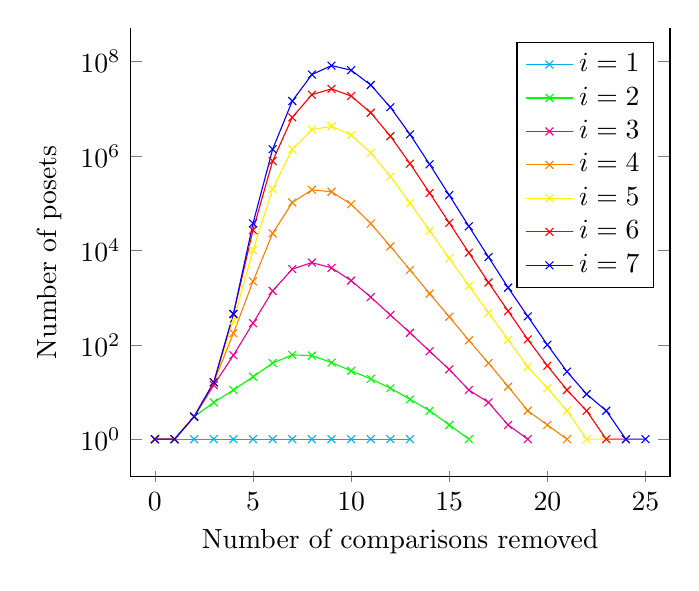
\begin{tikzpicture}
  \begin{axis}[
      ymode=log,
      axis x line = bottom,%x-Achse nur unten
      % x dir=reverse,
      enlarge x limits = .05,%x-Achse erweitern
      x axis line style = {-},%kein Pfeil
      % title = {\dots},
      ylabel={Number of posets},
      xlabel={Number of comparisons removed},
      % only marks,
      cycle list={{mark=x}},
      legend pos=north east,
    ]
    \addlegendentry{$i = 1$}
    \addplot+[cyan] table { %n=14,i=0
        x  y
        0  1
        1  1
        2  1
        3  1
        4  1
        5  1
        6  1
        7  1
        8  1
        9  1
        10 1
        11 1
        12 1
        13 1
      };
    \addlegendentry{$i = 2$}
    \addplot+[green] table { %n=14,i=1
        x y
        0  1
        1  1
        2  3
        3  6
        4  11
        5  21
        6  41
        7  61
        8  59
        9  42
        10 28
        11 19
        12 12
        13 7
        14 4
        15 2
        16 1
      };
    \addlegendentry{$i = 3$}
    \addplot+[magenta] table { %n=14,i=2
        x y
        0  1
        1  1
        2  3
        3  14
        4  60
        5  287
        6  1385
        7  4005
        8  5510
        9  4268
        10 2284
        11 1025
        12 428
        13 180
        14 73
        15 30
        16 11
        17 6
        18 2
        19 1
      };
    \addlegendentry{$i = 4$}
    \addplot+[orange] table { %n=14,i=3
        x y
        0  1
        1  1
        2  3
        3  16
        4  175
        5  2201
        6  22900
        7  103210
        8  191627
        9  174416
        10 94785
        11 37004
        12 12173
        13 3851
        14 1211
        15 392
        16 124
        17 41
        18 13
        19 4
        20 2
        21 1
      };
    \addlegendentry{$i = 5$}
    \addplot+[yellow] table { %n=14,i=4
        x y
        0  1
        1  1
        2  3
        3  16
        4  323
        5  10111
        6  200521
        7  1386176
        8  3607272
        9  4267576
        10 2763862
        11 1162696
        12 367875
        13 100552
        14 26024
        15 6745
        16 1781
        17 474
        18 127
        19 34
        20 12
        21 4
        22 1
        23 1
      };
    \addlegendentry{$i = 6$}
    \addplot+[red] table { %n=14,i=5
        x y
        0  1
        1  1
        2  3
        3  16
        4  446
        5  26921
        6  780123
        7  6588569
        8  19882832
        9  26416869
        10 18631911
        11 8243306
        12 2630332
        13 688904
        14 164372
        15 38334
        16 8918
        17 2084
        18 518
        19 130
        20 36
        21 11
        22 4
        23 1
        24 1
      };
    \addlegendentry{$i = 7$}
    \addplot+[blue] table { % n=14,i=6
        x y
        0  1
        1  1
        2  3
        3  16
        4  452
        5  37236
        6  1389385
        7  14591680
        8  53003482
        9  82198656
        10 65707713
        11 31909980
        12 10770689
        13 2864659
        14 665109
        15 147573
        16 32349
        17 7214
        18 1624
        19 400
        20 100
        21 27
        22 9
        23 4
        24 1
        25 1
      };
  \end{axis}
\end{tikzpicture}
    }
    \caption{Number of posets for $n = 14$ depending on the number of comparisons}
  \end{figure}
\end{frame}


\section{Results}
\sectionframe{\insertsection}

\begin{frame}{Exact Bounds} %ready
  \vspace{-1cm}
  \begin{table}[!t]
    \label{tab:results}
    \centering
    \small
    \begin{tabular}{c|cccccccc}
      $n$ & \multicolumn{8}{c}{$i$}                                                                                                      \\
          & 1                       & 2  & 3           & 4           & 5           & 6           & 7                 & 8                 \\ \hline
      1   & 0                                                                                                                            \\
      2   & 1                                                                                                                            \\
      3   & 2                       & 3                                                                                                  \\
      4   & 3                       & 4                                                                                                  \\
      5   & 4                       & 6  & 6                                                                                             \\
      6   & 5                       & 7  & 8                                                                                             \\
      7   & 6                       & 8  & 10          & 10                                                                              \\
      8   & 7                       & 9  & 11          & 12                                                                              \\
      9   & 8                       & 11 & 12          & 14          & 14                                                                \\
      10  & 9                       & 12 & 14          & 15          & 16                                                                \\
      11  & 10                      & 13 & 15          & 17          & 18          & 18                                                  \\
      12  & 11                      & 14 & 17          & 18          & 19          & 20                                                  \\
      13  & 12                      & 15 & 18          & 20          & 21          & 22          & 23                                    \\
      14  & 13                      & 16 & 19          & 21          & 23          & 24          & \textbf{25}                           \\
      15  & 14                      & 17 & 20          & 23          & \textbf{24} & \textbf{26} & \textbf{26}       & \textbf{27}       \\
      16  & 15                      & 18 & \textbf{21} & \textbf{24} & \textbf{26} & \textbf{27} & \textbf{28} -- 33 & \textbf{28} -- 36 \\
    \end{tabular}
  \end{table}
\end{frame}

\begin{frame}{Our Contribution}
  \definecolor{counterexample}{rgb}{0.8, 0.1, 0.1}
  \setbeamercolor{block title alerted}{bg=gray!20,fg=black}
  \setbeamercolor{block body alerted}{bg=gray!5}
  \begin{itemize}
    \item<+-> Verified existing results and generated executable algorithms
    \item<+-> Calculated and corrected new lower bounds
    \item<+-> Introduced compatible posets and backward search as novelty for this problem
    \item<+-> Disproved a conjecture on optimal algorithm structure from Gasarch:
      ``An optimal algorithm exists that first compares all elements pairwise.''
      \begin{alertblock}<+->{Counterexample: $n=12, i=5$}
        The conjecture implies a minimum of 20 comparisons are required. \\[0.5em]
        \textbf{Our discovered algorithm succeeds with only \textcolor{counterexample}{19} comparisons.}
      \end{alertblock}
  \end{itemize}
\end{frame}

\begin{frame}{Runtime Comparison} % ready
  \begin{table}[!t]
    \label{tab:times}
    \renewcommand{\arraystretch}{1.0}
    \centering
    \resizebox{1.0\textheight}{!}{%
      \begin{tabular}{c|c|l|l|l}
        $n$ & $i$ & \textbf{Forward Search} & \textbf{Backward Search} & \textbf{Oksanen}                                         \\
        \hline
        14  & 1   & 0.0s                    & 0.0s                     & 0.0s                                                     \\
        14  & 2   & 0.0s                    & 1.5s                     & 0.0s                                                     \\
        14  & 3   & 1.4s                    & 5.9s                     & \textbf{0.6s}                                            \\
        14  & 4   & \textbf{35.9s}          & 46.9s                    & 1m 47s                                                   \\
        14  & 5   & 17m 27s                 & \textbf{15m 33s}         & 6h 29m                                                   \\
        14  & 6   & 2h 40m                  & \textbf{1h 40m}          & 4d 10h                                                   \\
        14  & 7   & 14h 40m                 & \textbf{6h 27m}          & >5d                                                      \\
        \hline
        15  & 1   & 0.0s                    & 0.0s                     & 0.0s                                                     \\
        15  & 2   & 0.1s                    & 4.0s                     & \textbf{0.0s}                                            \\
        15  & 3   & 2.8s                    & 25.9s                    & \textbf{1.4s}                                            \\
        15  & 4   & \textbf{2m 24s}         & 13m 11s                  & 27m 17s                                                  \\
        15  & 5   & 1h 12m                  & \textbf{45m 52s}         & 1d 5h 40m\footnote{calculates a non-optimal lower bound} \\
        15  & 6   & 1d 8h 37m               & \textbf{19h 30m}         & >5d                                                      \\
        15  & 7   & 4d 23h 37m              & \textbf{1d 5h 43m}       & >5d                                                      \\
        15  & 8   & 14d 1h 51m              & \textbf{3d 8h 9m}        & >5d                                                      \\
      \end{tabular}
    }
  \end{table}
\end{frame}

\begin{frame}{Future Work}
  \vspace{-1.2cm}
  \begin{columns}
    \begin{column}{.49\textwidth}
      \begin{itemize}
        \item<+-> Idea of bidirectional Search: Run forward and backward search simultaneously
        \item<+-> Challenge: The searches intersect only after $> 99.9\%$ of the search space has been explored in both searches
        \item<+-> Forward search can prune subtrees, but the backward search needs to calculate the full tree
      \end{itemize}
    \end{column}
    \begin{column}{.49\textwidth}
      \onslide<2->{
        \begin{figure}[!b]
          \centering
          \renewcommand{\arraystretch}{0.9}
          \resizebox{0.85\textheight}{!}{%
            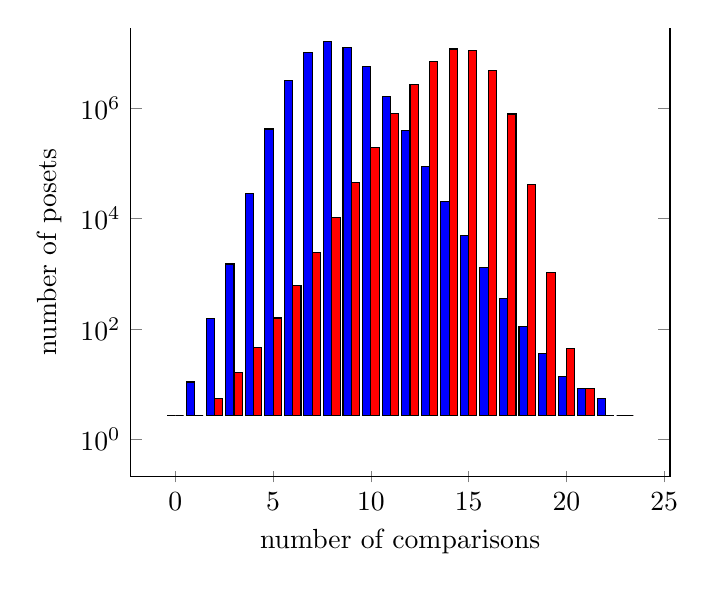
\begin{tikzpicture}
  \begin{axis}[
      ybar,
      ymode=log,
      axis x line = bottom,%x-Achse nur unten
      enlarge x limits = .1,%x-Achse erweitern
      x axis line style = {-},%kein Pfeil
      bar width=3pt,
      ylabel={number of posets},
      xlabel={number of comparisons},
      % legend cell align=left,
      % legend pos=outer north east,
      % legend style={at={(0.5,-0.2)},anchor=north}, % draw=none
    ]
    % \addlegendentry{forward search}
    \addplot[fill=blue,shift={(1pt, 0)}] table {
        x y
        0  1
        1  4
        2  57
        3  552
        4  10397
        5  154828
        6  1166640
        7  3770182
        8  5941732
        9  4726819
        10 2096404
        11 604582
        12 143058
        13 32460
        14 7450
        15 1823
        16 471
        17 132
        18 41
        19 13
        20 5
        21 3
        22 2
        23 1
      };
    % \addlegendentry{backward search}
    \addplot[fill=red,shift={(-1pt, 0)}] table {
        x y
        23 1
        22 1
        21 3
        20 16
        19 381
        18 15227
        17 290138
        16 1750707
        15 4058631
        14 4368185
        13 2592437
        12 1006071
        11 291970
        10 72346
        9  16728
        8  3898
        7  893
        6  227
        5  58
        4  17
        3  6
        2  2
        1  1
        0  1
      };
  \end{axis}
\end{tikzpicture}

Treff: 11
          }
          \caption{Poset distribution for $n = 13$, $i = 7$}
          \label{fig:backward_forward_count_13_6}
        \end{figure}
      }
    \end{column}
  \end{columns}
\end{frame}

% TODO: prevent in toc above
% \begin{frame}[shrink=25]{References}
%   \nocite{*}
%   \printbibliography[heading=none]
% \end{frame}

\thanksframe